% % include the figures path relative to the master file
% \graphicspath{ {./content/results/figures/} }

\section{Experiments and Validation}
\label{sec:exp} \label{sec:exp:datasets}

To evaluate the effects and influence of the different blocks composing our framework, an experimentation suit has been designed to test different configuration parameters evaluated in various datasets (see \cref{tab:experiment_summary}).
\begin{changebar}
Despite details regarding the data can be found in \cref{sec:exp:dataset:seri} and \cref{sec:exp:dataset:duke}; and specific details of the experiments can be fount in \cref{subsec:exp1} to \cref{subsec:exp4}; henceforth details the experimentation aspects and the design decisions that are consistent across all the experimentation.
\end{changebar}

Unless stated otherwise, all the experiments are run using our own dataset (SERI) alone.
Only for the sake of comparison some experiments are re-run on the Duke public dataset using our optimal configurations.

For all the experiments, \ac{lbp} and \ac{lbptop} features are extracted for different sampling points of 8, 16, and 24 for radius of 1, 2, and 3, respectively.
As previously mentioned, two different mapping strategies, \emph{local} and \emph{global}, are used, where for \emph{local} mapping, we consider a ($7 \times 7$) \acf{sw} for 2D \ac{lbp} and ($ 7 \times 7 \times 7$) sub-volume for \ac{lbptop}.

\deleted[id=sik]{ The pipeline in each experiment is }{All the experiments are} evaluated using \ac{lopocv} strategy.
In this validation, at each round a pair \ac{dme}-normal volume is selected for testing while the rest of the volumes are used for training.
The use of this method implies that no variance in terms of \ac{se} and \ac{sp} can be reported.
However, and despite this limitation, \ac{lopocv} has been employed due to the small size of the dataset.

The obtained results of all the experiments except experiment \#2 is represented in terms of \ac{se} and \ac{sp}.
All the experiments are evaluated in terms of \ac{se} and \ac{sp}, which are statistics driven from the confusion matrix (see Fig.~\ref{fig:CM}) as stated in \cref{eq:sesp}.
The \ac{se} evaluates the performance of the classifier with respect to the positive class, while the \ac{sp} evaluate it's performance with respect to negative class.
\begin{align}
 \ac{se}  = \frac{TP}{TP+FN} \qquad \ac{sp} = \frac{TN}{TN+FP}
 \label{eq:sesp}
\end{align}

Some experiments are complemented using \ac{acc} and \ac{f1}.
\acl{acc} is used to have a overall sense of classifier performance, and \ac{f1} is used to see the trade off between \ac{se} and precision.
Equation.~\ref{eq:accf1} shows the formulation of these two measurements. 
\begin{align}
\ac{acc} = \frac{TP+TN}{TP+TN+FP+FN} \qquad \ac{f1} = \frac{2TP}{2TP +FP+FN}
\label{eq:accf1}
\end{align}

\begin{figure}
\begin{center}
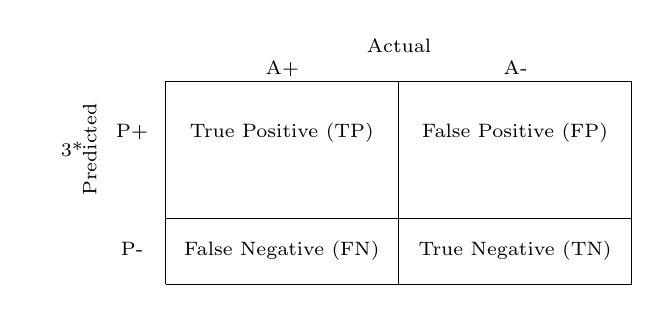
\begin{tikzpicture}[scale=0.4]
      \node at (1,1){
      \scriptsize{
        \begin{tabular}{
            >{\centering}m{1em} >{\centering}m{1em} >{\centering}m{1in} >{\centering\arraybackslash}m{1in}}
          % c>{\centering}m{2em}ccc}
          & & \multicolumn{2}{c}{ Actual}\\
          & & A+ & A- \\
          \cline{3-4}
          & \multicolumn{1}{c|}{} & \multicolumn{1}{c|}{} & \multicolumn{1}{c|}{}\\
          \multirow{3}{*}{\rotatebox[origin=c]{90}{Predicted}}& \multicolumn{1}{c|}{P+} &  \multicolumn{1}{c|}{True Positive (TP)} & \multicolumn{1}{c|}{False Positive (FP)} \\
          &\multicolumn{1}{c|}{}  & \multicolumn{1}{c|}{}& \multicolumn{1}{c|}{} \\
          \cline{3-4}
          & \multicolumn{1}{c|}{} &\multicolumn{1}{c|}{} & \multicolumn{1}{c|}{}\\
          
          & \multicolumn{1}{c|}{P-} &\multicolumn{1}{c|}{False Negative (FN)}  &\multicolumn{1}{c|}{True Negative (TN)}\\
          & \multicolumn{1}{c|}{} &\multicolumn{1}{c|}{} & \multicolumn{1}{c|}{}\\
          \cline{3-4}
          \end{tabular}
      }};
    \end{tikzpicture}
    \end{center}
\caption{Confusion matrix with truly and falsely positive detected samples (\acs{tp}, \acs{fp}) in the first row, from left to right and the falsely and truly negative detected samples (\acs{fn}, \acs{tn}) in the second row, from left to right.}
\label{fig:CM}
\end{figure}


Experimentation details can be fount in \cref{subsec:exp1} to \cref{subsec:exp4} and summarized in \cref{tab:experiment_summary}.
In general terms, all the experiments have been carried out using SERI dataset while \emph{Experiment \#1\,\cref{subsec:exp1}} has been complemented using Duke dataset for comparison purposes. This \emph{Experiment \#1\,\cref{subsec:exp1}} takes from the experimentation reported in \cite{Lemaintre2015miccaiOCT} to evaluate the effects of different feature representations\todo{are not we evaluating feature extraction?} and compares the results to those obtained by Venhuizen\emph{et al.}\,\cite{Venhuizen2015}.
\emph{Experiment \#2\,\cref{subsec:exp2}} studies the effect of the codebook size in order to find the optimal number of words for our application when using \ac{bow}.
\emph{Experiment \#3\,\cref{subsec:exp3}} studies the effect different pre-processing and classifiers.


\deleted[id=sik]{
The \emph{global} and \emph{local} extracted features are then presented in low or high level representation.
As previously mentioned, \ac{bow} approach is used for high-level representation.
% In this regard, to find the optimal number of  
}

\deleted[id=sik]{
Four experiments are presented in the reminder of this section.
Experiment \#1 presents the obtained results from our primary study~\cite{Lemaintre2015miccaiOCT} where we the framework was tested with one pre-processing, one classifier, and fixed number of visual words. 
In this regard in the next experiment \#2, we perform a preliminary test in a search for the optimal number of ``visual-words'' ($k$).
In experiment \#3, using the obtained number of words, we test the performance of different classifiers with regards to different pre-processing steps for high-level represented features and finally in experiment \#4 we compare the performance of different classifiers with respect to different pre-processing for low-level represented features.
%
\\
Beside experiment \#1, where the primary pipeline is tested on SERI and Duke dataset, the rest of the experiment are performed only on SERI dataset and for the sake of the comparison, these three experiments are performed using all the aforementioned classifiers. 
However only the relevant part and results related to our experiment is represented within the paper, while the rest are mentioned in online {\color{red}repository}.
}





\subsection{SERI-Dataset}\label{sec:exp:dataset:seri}
This data was acquired by Singapore Eye Research Institute (SERI), using CIRRUS TM (Carl Zeiss Meditec, Inc., Dublin, CA) \ac{sdoct} device. The datasets consist of 32 \ac{oct} volumes (16 \ac{dme} and 16 normal cases). Each volume contains 128 B-sane with  dimension of 512 $\times$ 1024 pixels.  All \ac{sdoct} images are read and assessed by trained graders and identifies as normal or \ac{dme} cases based on evaluation of retinal thickening, hard exudates, intraretinal cystoid space formation and subretinal fluid.

\subsection{Duke-Dataset} \label{sec:exp:dataset:duke}
This data published by Srinivasan\,\emph{et al.}~\cite{Srinivasan2014} was acquired in Institutional Review Board-approved protocols using Spectralis \ac{sdoct} (Heidelberg Engineering Inc., Heidelberg, Germany) imaging at Duke University, Harvard University and the University of Michigan. This datasets consist of 45 \ac{oct} volumes (15 \ac{amd}, 15 \ac{dme} and 15 normal). In this study we only consider a subset of the original data containing 15 \ac{dme} and 15 normal \ac{oct} volumes.


% \subsection{Experiments \& Results}
% The performed experiments are listed in the following:\\
%%Both datasets are filtered to attenuate the effect of speckle noise.
%%SIRE dataset is processed using \ac{nlm} as stated in Sect.\,\ref{subsec:prepro}.
%%The different parameters were empirically tested and fixed such that the patch size, the search window and the filtering parameter were set to $(15 \times 15)$, $(35 \times 35)$ and $0.4$, respectively.
%%However, Duke dataset is already filtered using BM3D method~\cite{Srinivasan2014}.
%%For both datasets, \ac{lbp} and \ac{lbptop} features are extracted for different sampling points of 8, 16 and 24 for radius of 1, 2 and 3, respectively.
%%Two different mapping strategies are used: (i) \emph{global} mapping corresponding to the 2D B-scan for \ac{lbp} or the 3D volume for \ac{lbptop} and (ii) \emph{local} mapping considering to a set of 2D \ac{sw} of size $(7 \times 7)$ for \ac{lbp} or the 3D sub-volume for \ac{lbptop} of size $(7 \times 7 \times 7)$.
\subsection{Experiment \#1}\label{subsec:exp1}
As previously stated, this experiment was performed with our primary framework which is presented in \cite{Lemaintre2015miccaiOCT}.
This experiment was performed to evaluate the effects of different features representation.
In this experiment, the \ac{oct} volumes of our own dataset, were only de-noised using \ac{nlm} method and \ac{bow} approach was used with fix number of words ($k = 32$).
Then the low or high level represented features were classified using \ac{rf} classifier with 100 un-pruned trees.  
For the sake of comparison, the same classification were performed for the extracted \emph{global} and \emph{local} \ac{lbptop}, and \emph{local}-\ac{lbp} features from Duke dataste.
As previously mentioned, this dataset is provided with cropped volumes, which vary in sizes.
Thus it was impossible to create a descriptor based on the \emph{global}-\ac{lbp} features for this dataset.
The obtained results from this experiment is listed in Table.~\ref{tab:table1-1}.

  \begin{table}[h]
\caption{ Experiment \#1 - Obtained results of classification using SERI and Duke datasets.}% using \ac{rf} with 100 trees. High-level features with \ac{bow} are obtained with $K$ = 32 visual-words.}
\centering
\resizebox{1\linewidth}{!}{

\begin{tabular}{l lr c lr c lr  c  lr c lr c lr}
\toprule
Features & \multicolumn{8}{c}{SERI dataset} & & \multicolumn{8}{c}{Duke dataset}\\
\cmidrule(l){2-9} \cmidrule(l){11-18}
 	& \multicolumn{2}{c}{$\{8,1\}$}& & \multicolumn{2}{c}{$\{16,2\}$}& &\multicolumn{2}{c}{$\{24,3\}$} & & \multicolumn{2}{c}{$\{8,1\}$}& & \multicolumn{2}{c}{$\{16,2\}$}& &\multicolumn{2}{c}{$\{24,3\}$}\\
  \cmidrule(l){2-3}  \cmidrule(l){5-6}  \cmidrule(l){8-9} \cmidrule(l){11-12}  \cmidrule(l){14-15}  \cmidrule(l){17-18}
	       & \ac{se} & \ac{sp} & & \ac{se} & \ac{sp} & &  \ac{se} & \ac{sp} & &  \ac{se} & \ac{sp} & &  \ac{se} & \ac{sp} & &  \ac{se} & \ac{sp} \\
\midrule
  	%\ac{lbp}					& 43.7 & 43.7 & & 37.5 & 50.0 & & 50.00 & 62.50  \\
 	\emph{global}-\ac{lbptop}				       & 56.2 & 62.5 & & \textbf{87.5} & \textbf{75.0} & & 68.7 & 68.7 & & 80.0 & 93.3 & & 73.3 & 86.6 & & 73.3 & 86.6 \\
	%\ac{lbp}+\ac{bow}		& 50.0 & 81.2 & & 57.5 & 68.7 & & 50.0 & 50.0 \\
	\emph{local}-\ac{lbp}	   & \textbf{75.0} & \textbf{87.5} & & 81.2 & 75.0 & & 68.7 & 62.5 & & \textbf{80.0} & \textbf{86.6} & & \textbf{86.7} & \textbf{100} & & 93.3 & 86.6\\
	\emph{local}-\ac{lbptop}   & 62.5 & 68.7 & & 56.2 & 37.5 & & 37.5 & 43.7 & & 80.0 & 86.6 & & 86.6 & 86.6 & & 60.0 & 80.0 \\
\bottomrule
\end{tabular}}
\label{tab:table1-1}
\end{table}






Once again in order to evaluate the proposed pipeline the proposed method by Venhuizen\,\textit{et al.}~\cite{Venhuizen2015} was developed and tested on the two dataset. The comparison of the obtained results with the highest performance achieved by our framework is shown in Table.~\ref{ta:table1-2}

\begin{table}[h]
\caption{Experiment \#1 - Comparing the proposed method by \cite{Venhuizen2015} on SERI and Duke datasets.}% with the \textbf{our two} best proposed methods. $K$ = 32 and \ac{rf} is trained using 100 tress}
\centering
\scriptsize{
\begin{tabular}{l	lr c lr}
\toprule
Data sets 	& \multicolumn{2}{c}{SERI} & & \multicolumn{2}{c}{Duke} \\
  \cmidrule(l){2-3}  \cmidrule(l){5-6}
	         & \ac{se} & \ac{sp} & & \ac{se} & \ac{sp}\\
\midrule
Venhuizen~\textit{et al.} \cite{Venhuizen2015} 		& 61.5 & 58.8 & & 71.4 & 68.7\\
\{\emph{local}-\ac{lbp}\},$\{8,1\}$				   & \textbf{75.0} & \textbf{87.5} & & \textbf{86.6} & \textbf{100.0}   \\
\{\emph{global}-\ac{lbptop}\},$\{16,2\}$				& \textbf{75.0} & \textbf{87.5} & & 80.0 & 86.6  \\


\bottomrule
\end{tabular}}
\label{tab:table1-2}
\end{table}
\label{subsec:exp2}

\subsection{Experiment \#2}
This experiment, conducted on SERI dataset, is performed to find the optimal number of words for \ac{bow} high-level feature representation.
\emph{Global} and \emph{local}-\ac{lbp} and \emph{local}-\ac{lbptop} feature descriptors are re-represented using \ac{bow} approach.
In this experiment, the \ac{bow} algorithm is performed using various number of words in the range of $\{10, 20, 30, \cdots,$
 $100, 200, \cdots, 500, 1000\}$.
The words are randomly selected using $k$-means++ algorithm and the features are mapped to their nearest word to create the final clusters.
In order to asses the effect of number of words, simple linear classifier such as \ac{lr} is used.
The number of words associated with highest \ac{acc} and \ac{f1} score, is selected as the optimum number of words.
Table~\ref{tab:table2} shows the obtained results of this experiment.
The optimum number of words and the achieved \ac{acc} and \ac{f1} of \ac{lr} classifier for different configurations are listed in this table.


\begin{landscape}

  \begin{table}
\caption{Experiment \#1 - Optimum number of words for each configuration as a result of \ac{lr} Classification, for high-level feature extraction of \emph{global} and \emph{local}-\ac{lbp}, and \emph{local}-\ac{lbptop} features with different pre-processing. The pre-processing includes: \ac{nf}, \ac{f}, and \ac{fal}.
The achieved performances are indicated in terms of  \acs{acc}, \acs{f1}, \acs{se}, and \acs{sp}}
\centering

\footnotesize{
\resizebox{1\linewidth}{!}{
\begin{tabular}{ll  ccccr	c	ccccr	c ccccr}
\toprule
Features & Pre-processing &    \multicolumn{5}{c}{$\{8,1\}$}  & & \multicolumn{5}{c}{$\{16,2\}$} & & \multicolumn{5}{c}{$\{24,3\}$} \\
  \cmidrule(l){3-7}  \cmidrule(l){9-13}  \cmidrule(l){15-19}
   & &  	\ac{acc}\% & \ac{f1}\% & \ac{se}\% & \ac{sp}\%  & W\# &  & \ac{acc}\% & \ac{f1}\% & \ac{se}\% & \ac{sp}\%  & W\# &  &\ac{acc}\% & \ac{f1}\% & \ac{se}\% & \ac{sp}\%  & W\# \\
\midrule
\\[-2ex]
  	\emph{global}-\ac{lbp}		\\
 	& \acs{nf} & 81.2 &  78.5 & 68.7 &  93.7 & 500 & & 62.5 & 58.0 & 56.2 & 62.5 & 80  & & 62.5  & 62.5 & 62.5 & 62.5 & 80  \\
	& \acs{f}  & 71.9 &  71.0 & 68.7 &  75.0 & 400 & & 68.7 & 66.7 & 62.5 & 75.0 & 300 & & 68.7  & 66.7 & 62.5  & 75.0 & 300	 \\
	& \acs{fal}& 71.9 &  71.0 & 68.7 &  75.0 & 500 & & 71.9 & 71.0 & 68.7 & 75.0 & 200 & & 75.0  & 68.7 & 68.7  & 68.7 & 500	 \\
	%& \acs{fac}& 75.0 & 73.3 & 68.7 &  81.2 & 500 & & 78.1 & 75.8 & 68.7 & 87.5 & 500 & & 68.7  & 68.7 & 68.7  & 68.7 & 90	 \\
	\\
\hdashline \noalign{\vskip 3pt}
\\[-2ex]
 	\emph{local}-\ac{lbp}		\\
 	& \acs{nf}  &\cellcolor[gray]{0.6}75.0  &\cellcolor[gray]{0.6} 75.0 &\cellcolor[gray]{0.6} 75.0  &\cellcolor[gray]{0.6} 75.0 &\cellcolor[gray]{0.6} 70 & & 65.6 & 64.5 & 62.5 & 68.7 & 90 & &  62.5 & 60.0 & 56.2  & 68.7  & 30  \\
	& \acs{f}   & 75.0  & 73.3 & 68.7  & 81.2 & 30 & & 71.8 & 61.0 & 68.7 & 75.0 & 70 & &  62.5 & 62.5 & 62.5  & 62.5  & 100	 \\
	& \acs{fal} & 75.0  & 69.0 & 62.5  & 81.2 & 40 & & 71.9 & 71.0 & 68.7 & 75.0 & 200 & &  68.7 & 66.7 & 68.7 & 62.5 & 10	 \\
	%& \acs{fac}& 68.7 & 68.7 & 68.7 & 68.7 & 300 & & 65.6 & 64.5 & 62.5 & 68.7 & 100 & & 65.6  & 64.5 & 62.5  & 68.7 & 100	 \\
	\\
\hdashline \noalign{\vskip 3pt}
\\[-2ex]
 	\emph{local}-\ac{lbptop}		\\
 	& \acs{nf}	& 68.7 & 68.7 & 68.7 & 68.7 & 400 & & \cellcolor[gray]{0.6}75.0  & \cellcolor[gray]{0.6}75.0   &\cellcolor[gray]{0.6}75.0   &\cellcolor[gray]{0.6}75.0  &\cellcolor[gray]{0.6}500 & & 71.9 & 71.0 & 68.7 & 75.0 & 60	 \\
	& \acs{f}	& 68.7 & 68.7 & 68.7 & 68.7 & 300 & & 68.7  & 66.7   & 62.5   & 75.0  & 50  & & 75.0 & 76.5 & 81.2 & 68.7 & 80	 \\
	& \acs{fal}	& 75.0 & 73.3 & 68.7 & 81.2 & 100 & & 75.0  & 73.3   & 68.7   & 81.2  & 90  & & 75.0 & 69.0 & 62.5 & 81.2 & 70	 \\
	%& \acs{fac}	& 71.9 & 69.0 & 62.5 & 81.2 & 400 & & 75.0  & 73.3   & 68.7   & 81.2  & 100 & & 75.0 & 73.3 & 68.7 & 81.2 & 60	 \\
	\\

\bottomrule
\end{tabular}}}
\label{tab:table2}
\end{table}
\end{landscape}




Figure.~\ref{fig:RBOW} shows the obtained graphs for some of the configurations. \\

\begin{figure}[t]
  \missingfigure{fig:RBOW}
  \caption{}
  \label{fig:RBOW}
\end{figure}
 
\subsection{Experiment \#3}\label{subsec:exp3}
This experiment is performed for high-level features on SERI dataset. 
Using the optimum number of words which are obtained from the previous experiment, the low-level feature sets with regards to different pre-processing configurations are re-represented using \ac{bow} and $k$-means clustering approach and are classified using different classifiers such as $k$-\ac{nn}, \ac{rf}, \ac{gb}, and \ac{svm}.\
The $k$-means algorithm is initialized using $k$-means++ method and is performed with 5 iteration for each codebook.
The \ac{rf} and \ac{gb} classifier are trained using 100 un-pruned trees, while \ac{svm} classifier is trained with \ac{rbf} kernel. 
The regularization and soft-margin parameters of this classifier are chosen with grid-search method.
Finally the $k$-\ac{nn} classifier is trained by considering the 3 nearest neighbor.
Table~\ref{tab:table3} shows the obtained results from this experiment.\\

\begin{landscape}

  \begin{table}[ht]
\caption{Experiment \#3 - $k$-\ac{nn} and  \ac{svm} classification with \ac{bow} for the \emph{global} and \emph{local} \ac{lbp} and \emph{local} \ac{lbptop} features with different pre-processing. The optimum number of words were selected based on the previous experiment.}
\centering

\scriptsize{
\resizebox{0.9\linewidth}{!}{
\begin{tabular}{ll  lr	c	lr	c lr c lr	c	lr	c lr}
\toprule
& & \multicolumn{8}{c}{$k$-\ac{nn}} & & \multicolumn{8}{c}{\ac{svm}}\\
\cmidrule(l){3-10} \cmidrule(l){12-19}
Features & Pre-processing &    \multicolumn{2}{c}{$\{8,1\}$}  & & \multicolumn{2}{c}{$\{16,2\}$} & & \multicolumn{2}{c}{$\{24,3\}$}  & &   \multicolumn{2}{c}{$\{8,1\}$}  & & \multicolumn{2}{c}{$\{16,2\}$} & & \multicolumn{2}{c}{$\{24,3\}$} \\
  \cmidrule(l){3-4}  \cmidrule(l){6-7}  \cmidrule(l){9-10}   \cmidrule(l){12-13}  \cmidrule(l){15-16}  \cmidrule(l){18-19}
   & &  	\ac{se}\% & \ac{sp}\% &  & \ac{se}\% & \ac{sp}\% &  & \ac{se}\% & \ac{sp}\%  & & 	\ac{se}\% & \ac{sp}\% &  & \ac{se}\% & \ac{sp}\% &  & \ac{se}\% & \ac{sp}\% \\
\midrule
  	\emph{global}-\ac{lbp}		\\
 	& \acs{nf} & 43.7 &  93.7 &   & 43.7 & 87.5  &  & 43.7  & 62.5  &  & 68.7 & 87.5 & & 62.5 & 62.5 & & 50.0 & 56.2 \\  
	& \acs{f}  & 43.7 &  56.2 &   & 50.0 & 75.0  &  & 62.5  & 56.2  &  & 56.2 & 56.2 & & 56.2 & 75.0 & & 56.2 & 68.7  \\
	& \acs{fa} & 56.2 &  62.5 &   & 43.7 & 81.2  &  & 68.7  & 56.2  &  & 56.2 & 68.7 & & 68.7 & 68.7 & & 56.2 & 75.0	 \\
	%& \acs{fac}& 50   &  75.0 &   & 37.5 & 87.5  &  & 50.0  & 62.5 &  & 50.0 & 75.0 & & 50.0 & 75.0 & & 43.7 & 68.7 \\
\hdashline \noalign{\vskip 3pt}
 	\emph{local}-\ac{lbp}		\\
 	& \acs{nf} & \cellcolor[gray]{0.8}\textbf{75.0} & \cellcolor[gray]{0.8}\textbf{87.5} & & 50.0  & 68.7 &  &  43.7  & 43.7 & & \cellcolor[gray]{0.6}\textbf{75.0} & \cellcolor[gray]{0.6}\textbf{93.7} & & 50.0 & 75.0 & & 56.2 & 56.2    \\
	& \acs{f}  & \cellcolor[gray]{0.8}56.2 & \cellcolor[gray]{0.8}56.2 & & 50.0  & 50.0 &  & 50.0   & 43.7 & &\cellcolor[gray]{0.6}\textbf{81.2} & \cellcolor[gray]{0.6}\textbf{93.7} & & 68.7 & 68.7 & & 68.7 & 75.0 \\
	& \acs{fa} & \cellcolor[gray]{0.8}56.2 & \cellcolor[gray]{0.8}43.7 & & 50.0  & 75.0 &  & 50.0   & 62.5 & & \cellcolor[gray]{0.6}\textbf{75.0} & \cellcolor[gray]{0.6}\textbf{93.7} & & 75.0 & 68.7 & & 68.7 & 68.7  \\
	%& \acs{fac}& 37.5 & 75.0 & & 31.2 & 75.0 &  & 62.5  & 81.2 & & 62.5 & 87.5 & & 56.2 & 43.7 & & 75.0 & 56.2	 \\
\hdashline \noalign{\vskip 3pt}
 	\emph{local}-\ac{lbptop}		\\
 	& \acs{nf} & 56.2 & 75.0 & & 56.2 & 75.0 & & 62.5 & 56.2 & & \cellcolor[gray]{0.8}\textbf{81.2} & \cellcolor[gray]{0.8}\textbf{87.5} & & \cellcolor[gray]{0.8}\textbf{75.0} & \cellcolor[gray]{0.8}\textbf{100} & & 56.2 & 75.0 \\
	& \acs{f} & 62.5 & 43.7 & & 37.5 & 68.7 & & 43.7 & 62.5 & & \cellcolor[gray]{0.8}\textbf{81.2} & \cellcolor[gray]{0.8}\textbf{81.2} & & \cellcolor[gray]{0.8}75.0 & \cellcolor[gray]{0.8}68.7 & & 81.2 & 68.7		 \\
	& \acs{fal}	& 56.2 & 56.2 & & 68.7 & 50.0 & & 43.7 & 62.5 & & \cellcolor[gray]{0.8}62.5 & \cellcolor[gray]{0.8}75.0 & & \cellcolor[gray]{0.8}68.7 & \cellcolor[gray]{0.8}75.0 & & 62.5 & 81.2  \\
	%& \acs{fac} & 43.7 & 68.7 & & 68.7 & 75.0 & & 56.2 & 81.2 & & 56.2 & 87.5 & & 87.5 & 75.0 & & 62.5 & 75.0	 	 \\
\midrule
& & \multicolumn{8}{c}{\ac{rf}} & & \multicolumn{8}{c}{\ac{gb}}\\
\cmidrule(l){3-10} \cmidrule(l){12-19}
Features & Pre-processing &    \multicolumn{2}{c}{$8^{riu2}$}  & & \multicolumn{2}{c}{$16^{riu2}$} & & \multicolumn{2}{c}{$24^{riu2}$}  & &   \multicolumn{2}{c}{$8^{riu2}$}  & & \multicolumn{2}{c}{$16^{riu2}$} & & \multicolumn{2}{c}{$24^{riu2}$} \\
  \cmidrule(l){3-4}  \cmidrule(l){6-7}  \cmidrule(l){9-10}   \cmidrule(l){12-13}  \cmidrule(l){15-16}  \cmidrule(l){18-19}
   & &  	\ac{se}\% & \ac{sp}\% &  & \ac{se}\% & \ac{sp}\% &  & \ac{se}\% & \ac{sp}\%  & & 	\ac{se}\% & \ac{sp}\% &  & \ac{se}\% & \ac{sp}\% &  & \ac{se}\% & \ac{sp}\% \\
\midrule
  	\emph{global}-\ac{lbp}		\\
 	& \acs{nf} & \cellcolor[gray]{0.8}\textbf{68.7} & \cellcolor[gray]{0.8}\textbf{93.7} & & 43.7 & 62.5 & & 50.0 & 68.7  & & 56.2 & 50.0 & & 37.5 & 31.2 & & 50.0 & 43.7\\
	& \acs{f}  & \cellcolor[gray]{0.8}56.2 & \cellcolor[gray]{0.8}50.0 & & 56.2 & 75.0 & & 50.0 & 75.0  & & 50.0 & 56.2 & & 56.2 & 75.0 & & 43.7 & 62.5\\
	& \acs{fa} & \cellcolor[gray]{0.8}68.7 & \cellcolor[gray]{0.8}50.0 & & 56.2 & 62.5 & & 62.5 & 56.2  & & 56.2 & 50.0 & & 68.7 & 50.0 & & 43.7 & 75.0\\
	%& \acs{fac} & 68.7 & 68.7 & & 56.2 & 75.0 & & 50.0 & 68.7& &  50.0 & 68.7 & & 75.0 & 62.5 & & 56.2 & 81.2  \\ 
\hdashline \noalign{\vskip 3pt}
 	\emph{local}-\ac{lbp}		\\
 	& \acs{nf} &  \cellcolor[gray]{0.8}\textbf{81.2} & \cellcolor[gray]{0.8}\textbf{81.2} & & 62.5 & 56.2 & & 56.2 & 56.2 & & 75.0 & 62.5 & & 68.7 & 87.5 & & 50.0 & 75.0   \\
	& \acs{f}  &  \cellcolor[gray]{0.8}56.2 & \cellcolor[gray]{0.8}81.2 & & 62.5 & 68.7 & & 68.7 & 62.5 & & 68.7 & 75.0 & & 50.0 & 75.0 & & 50.0 & 62.5 \\
	& \acs{fa} &  \cellcolor[gray]{0.8}68.7 & \cellcolor[gray]{0.8}62.5 & & 62.6 & 68.7 & & 43.7 & 43.7 & & 56.2 & 50.0 & & 68.7 & 56.2 & & 50.0 & 50.0 \\
	%& \acs{fac}&  62.5 & 68.7 & & 68.7 & 68.7 & & 68.7 & 56.2 & &  56.2 & 50.0 & & 56.2 & 68.7 & & 62.5 & 68.7  \\
\hdashline \noalign{\vskip 3pt}
 	\emph{local}-\ac{lbptop}		\\
 	& \acs{nf} & 68.7 & 62.5 & & \cellcolor[gray]{0.6}\textbf{68.7} & \cellcolor[gray]{0.6}\textbf{81.2} & & 68.7 & 68.7 & & 37.5 & 68.7 & & 62.5 & 81.2 & & 62.5 & 50.0  \\
	& \acs{f} & 50.0 & 62.5 & & \cellcolor[gray]{0.6}62.5 & \cellcolor[gray]{0.6}62.5 & & 43.7 & 75.0 & & 50.0 & 56.2 & & 43.7 & 62.5 & & 50.0 & 62.5		 \\
	& \acs{fal}	& 50.0 & 62.5 & & \cellcolor[gray]{0.6}\textbf{81.2} & \cellcolor[gray]{0.6}\textbf{87.5} & & 50.0 & 68.7 & & 56.2 & 62.5 & & 81.2 & 68.7 & & 75.0 & 68.7  \\
	%& \acs{fac}	 & 56.2 & 81.2 & & 68.2 & 81.2 & & 68.7 & 87.5 & & 75.0 & 68.7 & & 87.5 & 75.0 & & 75.0 & 87.5 	 \\

\bottomrule
\end{tabular}}}
\label{tab:table3}
\end{table}
%\end{tiny}
\end{landscape}

%--------------------------------------------------------
%  \begin{table}[ht]
%\caption{The obtained results of experiment \#2.
%Classification results obtained from low-level representation of global \ac{lbp} and \ac{lbptop} features with different pre-processing.
%Pre-processing steps include: \ac{nf}, \ac{f}, \ac{fal}, and \ac{fac}.
%Different classifiers such as \ac{rf}, \ac{gb}, \ac{svm}, \ac{lr}, and $k$-\ac{nn} are used.
%}
%\medskip
%
%\footnotesize{
%\begin{center}
%\resizebox{1\linewidth}{!}{
%%\begin{tabularx}{1.02\linewidth}{l cc  cc cc c cc cc cc }
%\begin{tabular}{l cc  cc cc c cc cc cc }
%\toprule
%& \multicolumn{6}{c}{\ac{rf}} & &  \multicolumn{6}{c}{\ac{gb}} \\
%\cmidrule(l){2-7} \cmidrule(l){9-14}
%Features &  \multicolumn{2}{c}{$8^{riu2}$}  & \multicolumn{2}{c}{$16^{riu2}$} & \multicolumn{2}{c}{$24^{riu2}$} & &  
%   \multicolumn{2}{c}{$8^{riu2}$}  &  \multicolumn{2}{c}{$16^{riu2}$} & \multicolumn{2}{c}{$24^{riu2}$} \\
%  \cmidrule(l){2-3}  \cmidrule(l){4-5}  \cmidrule(l){6-7} \cmidrule(l){9-10}  \cmidrule(l){11-12}  \cmidrule(l){13-14}
%   &  	\ac{se}\% &  \ac{sp}\%  &  \ac{se}\% &  \ac{sp}\% & 	\ac{se}\% &  \ac{sp}\% & & 
%   \ac{se}\% &  \ac{sp}\% & \ac{se}\% &  \ac{sp}\% & \ac{se}\% &  \ac{sp}\%\\
%\midrule
%  	\emph{global}-\ac{lbp} \\
% 	\acs{nf} & 43.7 & 62.5 &   43.7 & 62.5 & 56.2 & 75   & &  43.7 & 43.7 & 43.7 & 37.5 & 37.5 & 31.25  		\\
%	\acs{f}  & 56.2 & 56.2 &   68.7 & 62.5 & 62.5 & 68.7 & &  25   & 56.2 & 50   & 43.7 & 25   & 43.7 \\
%	\acs{fa} & 65.2 & 56.2 &   50   & 50   & 56.2 & 68.7 & &  43.75& 62.5 & 62.5 & 50   & 31.2 & 31.2 \\
%	\acs{fac}& 56.2 & 62.5 &   56.2 & 62.5 & 68.7 & 56.2 & &  25   & 62.5 & 75   & 81.2 & 93.7 & 87.5\\
%
%\hdashline \noalign{\vskip 3pt}
% 	\emph{global}-\ac{lbptop}		\\
% 	\acs{nf}	 & 56.2 & 68.7 &   68.7  & 87.5 & 68.7  & 81.2 & &  68.7 & 68.7 & 75   & 50   & 56.2 & 43.7\\
%	\acs{f}	 & 56.2 & 62.5 &   81.2  & 68.7 & 81.2  & 81.2 & &  56.2 & 62.5 & 62.5 & 68.7 & 68.7 & 81.2\\
%	\acs{fal}& 68.7 & 62.5 &   75    & 68.7 & 75    & 81.2 & &  56.2 & 43.7 & 62.5 & 62.5 & 75   & 75 \\
%	\acs{fac}& 75   & 68.7 &   75    & 81.2 & 75    & 75   & &  75   & 75   & 75   & 56.2 & 81.2 & 62.5\\
%\midrule
%& \multicolumn{6}{c}{\ac{svm}} & &  \multicolumn{6}{c}{$k$-\ac{nn}} \\
%\cmidrule(l){2-7} \cmidrule(l){9-14}
%Features &  \multicolumn{2}{c}{$8^{riu2}$}  & \multicolumn{2}{c}{$16^{riu2}$} & \multicolumn{2}{c}{$24^{riu2}$} & &  
%   \multicolumn{2}{c}{$8^{riu2}$}  &  \multicolumn{2}{c}{$16^{riu2}$} & \multicolumn{2}{c}{$24^{riu2}$} \\
%  \cmidrule(l){2-3}  \cmidrule(l){4-5}  \cmidrule(l){6-7} \cmidrule(l){9-10}  \cmidrule(l){11-12}  \cmidrule(l){13-14}
%   &  	\ac{se}\% &  \ac{sp}\%  &  \ac{se}\% &  \ac{sp}\% & 	\ac{se}\% &  \ac{sp}\% & & 
%   \ac{se}\% &  \ac{sp}\% & \ac{se}\% &  \ac{sp}\% & \ac{se}\% &  \ac{sp}\%\\
%\midrule
%  	\emph{global}-\ac{lbp}		\\
% 	\acs{nf} & 56.2 & 62.5 & 56.2 & 43.7 & 56.2 & 68.7 & & 37.5 & 50   & 25   & 50   & 37.5 & 68.7 \\
%	\acs{f}  & 75   & 68.7 & 62.5 & 62.5 & 62.5 & 68.7 & & 62.5 & 50   & 56.2 & 75   & 62.5 & 68.7\\
%	\acs{fa} & 75   & 68.7 & 62.5 & 62.5 & 62.5 & 68.7 & & 56.2 & 50   & 56.2 & 75   & 62.5 & 68.7 \\
%	\acs{fac}& 56.2 & 62.5 & 25   & 50   & 43.7 & 62.5 & & 50   & 43.7 & 68.7 & 62.5 & 62.5 & 62.5\\
%
%\hdashline \noalign{\vskip 3pt}
% 	\emph{global}-\ac{lbptop}		\\
% 	\acs{nf}	  & 62.5 & 75   & 62.5 & 93.7 & 56.2 & 87.5 & & 31.2 & 93.7 & 37.5 & 100  & 37.5 & 81.2 \\
%	\acs{f}	  & 68.7 & 75   & 43.7 & 68.7 & 68.7 & 56.2 & & 50   & 56.2 & 56.2 & 75   & 56.2 & 62.5\\
%	\acs{fal} & 68.7 & 62.5 & 62.5 & 56.2 & 56.2 & 68.7 & & 75   & 43.7 & 56.2 & 43.7 & 68.7 & 50  \\
%	\acs{fac} & 68.7 & 68.7 & 68.7 & 87.5 & 68.7 & 87.5 & & 62.5 & 62.5 & 68.7 & 68.7 & 75   & 75\\
%%\midrule
%%
%%& \multicolumn{6}{c}{\ac{lr}} \\
%%\cmidrule(l){2-7} 
%%Features &  \multicolumn{2}{c}{$8^{riu2}$}  & \multicolumn{2}{c}{$16^{riu2}$} & \multicolumn{2}{c}{$24^{riu2}$}  \\
%%  \cmidrule(l){2-3}  \cmidrule(l){4-5}  \cmidrule(l){6-7} 
%%   &  	\ac{se}\% &  \ac{sp}\%  &  \ac{se}\% &  \ac{sp}\% & 	\ac{se}\% &  \ac{sp}\% \\
%%\midrule
%%
%%\emph{global}-\ac{lbp}		\\
%%	\acs{nf}	  & 56.2 & 43.7 & 43.7 & 56.2 & 50 & 68.7\\
%%	\acs{f}	  & 56.2 & 43.7 & 56.2 & 37.5 & 68.7 & 43.7 \\
%%	\acs{fal} & 56.2 & 43.7 & 56.2 & 31.2 & 68.7 & 43.7 \\
%%	\acs{fac} & 62.5 & 56.2 & 56.2 & 62.5 & 56.2 & 56.2\\
%%
%%
%%\hdashline \noalign{\vskip 3pt}
%% 	\emph{global}-\ac{lbptop}		\\
%% 	\acs{nf}  & 50   & 50 &  6 & 93.7 & 0 & 100	\\
%%	\acs{f}	  & 75   & 18 & 50 & 75 & 25 & 81.2\\
%%	\acs{fal} & 93.7 & 6  & 93.7 & 6 & 50 & 43.7\\
%%	\acs{fac} & 50   & 81.2 & 0 & 93.7 & 0 & 100\\
%
%\bottomrule
%
%
%\end{tabular}}
%
%\end{center}}
%\label{tab:table4}
%\end{table}


\subsection{Experiment \#4}\label{subsec:exp4}
This experiment is conducted for low-level features.
The \emph{global} \ac{lbp} and \ac{lbptop} features are classified using the same classifiers as previous experiments with the same configurations.
The obtained results from this experiment is listed in Table.~\ref{tab:table4}.\\
\begin{landscape}

  \begin{table}[ht]
\caption{Experiment \#3 - Classification results obtained from low-level representation of global \ac{lbp} and \ac{lbptop} features with different pre-processing.
Pre-processing steps include: \ac{nf}, \ac{f}, \ac{fal}.
Different classifiers such as \ac{rf}, \ac{gb}, \ac{svm}, and $k$-\ac{nn} are used.
The most relevant configurations are shaded and the highest results are highlighted in \textbf{bold}.
The configurations which their performances declines with additional pre-processing are shaded in light gray while those with the opposite behavior are shaded with darker gray color.}

\medskip

\scriptsize{
\begin{center}
\resizebox{1\linewidth}{!}{
%\begin{tabularx}{1.02\linewidth}{l cc  cc cc c cc cc cc }
\begin{tabular}{ll cc  cc cc c cc cc cc }
\toprule
&  & \multicolumn{6}{c}{$k$-\ac{nn}} & &  \multicolumn{6}{c}{\ac{svm}} \\
\cmidrule(l){3-8} \cmidrule(l){10-15}
Features & Pre-processing &   \multicolumn{2}{c}{$\{8,1\}$}  & \multicolumn{2}{c}{$\{16,2\}$} & \multicolumn{2}{c}{$\{24,3\}$} & &  
   \multicolumn{2}{c}{$\{8,1\}$}  &  \multicolumn{2}{c}{$\{16,2\}$} & \multicolumn{2}{c}{$\{24,3\}$} \\
  \cmidrule(l){3-4}  \cmidrule(l){5-6}  \cmidrule(l){7-8} \cmidrule(l){10-11}  \cmidrule(l){12-13}  \cmidrule(l){14-15}
   &  & 	\ac{se}\% &  \ac{sp}\%  &  \ac{se}\% &  \ac{sp}\% & 	\ac{se}\% &  \ac{sp}\% & & 
   \ac{se}\% &  \ac{sp}\% & \ac{se}\% &  \ac{sp}\% & \ac{se}\% &  \ac{sp}\%\\
\midrule
  	\emph{global}-\ac{lbp}		\\
 	& \acs{nf} & 37.5 & 50.0   & 25.0 & 50.0   & 37.5 & 68.7 & & 56.2 & 62.5 & 56.2 & 43.7 & 56.2 & 68.7 \\
	& \acs{f}  & 62.5 & 50.0   & 56.2 & 75.0   & 62.5 & 68.7 & & 75.0 & 68.7 & 62.5 & 62.5 & 62.5 & 68.7 \\
	& \acs{fa} & 56.2 & 50.0   & 56.2 & 75.0   & 62.5 & 68.7 & & 75.0 & 68.7 & 62.5 & 62.5 & 62.5 & 68.7 \\
	%\acs{fac}& 50   & 43.7 & 68.7 & 62.5 & 62.5 & 62.5 & & 56.2 & 62.5 & 25   & 50   & 43.7 & 62.5  \\

\hdashline \noalign{\vskip 3pt}
 	\emph{global}-\ac{lbptop}		\\
 	& \acs{nf}	  &  31.2 & 93.7 & 37.5 & 100.0  & 37.5 & 81.2 & &  62.5 & 75.0   & \cellcolor[gray]{0.8}\textbf{62.5} & \cellcolor[gray]{0.8}\textbf{93.7} & 56.2 & 87.5  \\
	& \acs{f}	  &  50.0 & 56.2 & 56.2 & 75.0   & 56.2 & 62.5 & &  68.7 & 75.0   & \cellcolor[gray]{0.8}43.7 & \cellcolor[gray]{0.8}68.7 & 68.7 & 56.2 \\
	& \acs{fal}   &  75.0 & 43.7 & 56.2 & 43.7   & 68.7 & 50.0 & &  68.7 & 62.5   & \cellcolor[gray]{0.8}62.5 & \cellcolor[gray]{0.8}56.2 & 56.2 & 68.7  \\
	%\acs{fac} & 68.7 & 68.7 & 68.7 & 87.5 & 68.7 & 87.5 & & 62.5 & 62.5 & 68.7 & 68.7 & 75   & 75\\	
\midrule	
&  & \multicolumn{6}{c}{\ac{rf}} & &  \multicolumn{6}{c}{\ac{gb}} \\
\cmidrule(l){3-8} \cmidrule(l){10-15}
Features & Pre-processing &   \multicolumn{2}{c}{$8^{riu2}$}  & \multicolumn{2}{c}{$16^{riu2}$} & \multicolumn{2}{c}{$24^{riu2}$} & &  
   \multicolumn{2}{c}{$8^{riu2}$}  &  \multicolumn{2}{c}{$16^{riu2}$} & \multicolumn{2}{c}{$24^{riu2}$} \\
  \cmidrule(l){3-4}  \cmidrule(l){5-6}  \cmidrule(l){7-8} \cmidrule(l){10-11}  \cmidrule(l){12-13}  \cmidrule(l){14-15}
   & &  	\ac{se}\% &  \ac{sp}\%  &  \ac{se}\% &  \ac{sp}\% & 	\ac{se}\% &  \ac{sp}\% & & 
   \ac{se}\% &  \ac{sp}\% & \ac{se}\% &  \ac{sp}\% & \ac{se}\% &  \ac{sp}\%\\
\midrule
  	\emph{global}-\ac{lbp} \\
 	& \acs{nf} & 43.7 & 62.5 &   43.7 & 62.5 & 56.2 & 75   & &  43.7 & 43.7 & 43.7 & 37.5 & 37.5 & 31.25  		\\
	& \acs{f}  & 56.2 & 56.2 &   68.7 & 62.5 & 62.5 & 68.7 & &  25   & 56.2 & 50.0   & 43.7 & 25.0   & 43.7 \\
    & \acs{fal} & 65.2 & 56.2 &   50.0   & 50.0   & 56.2 & 68.7 & &  43.75& 62.5 & 62.5 & 50.0   & 31.2 & 31.2 \\
	%& \acs{fac}& 56.2 & 62.5 &   56.2 & 62.5 & 68.7 & 56.2 & &  25   & 62.5 & 75   & 81.2 & 93.7 & 87.5\\

\hdashline \noalign{\vskip 3pt}
 	\emph{global}-\ac{lbptop}		\\
 	& \acs{nf}	 & 56.2 & 68.7 &   \cellcolor[gray]{0.8}\textbf{68.7}  & \cellcolor[gray]{0.8}\textbf{87.5} & \cellcolor[gray]{0.6}\textbf{68.7}  & \cellcolor[gray]{0.6}\textbf{81.2} & &  68.7 & 68.7 & 75.0   & 50.0   & \cellcolor[gray]{0.8}56.2 & \cellcolor[gray]{0.8}43.7\\
	& \acs{f}	 & 56.2 & 62.5 &   \cellcolor[gray]{0.8}81.2  & \cellcolor[gray]{0.8}68.7 & \cellcolor[gray]{0.6}\textbf{81.2}  & \cellcolor[gray]{0.6}\textbf{81.2} & &  56.2 & 62.5 & 62.5 & 68.7 & \cellcolor[gray]{0.8}68.7 & \cellcolor[gray]{0.8}81.2\\
	& \acs{fal}& 68.7 & 62.5 &   \cellcolor[gray]{0.8}75.0    & \cellcolor[gray]{0.8}68.7 & \cellcolor[gray]{0.6}\textbf{75.0}   & \cellcolor[gray]{0.6}\textbf{81.2} & &  56.2 & 43.7 & 62.5 & 62.5 &\cellcolor[gray]{0.8}\textbf{75.0}   & \cellcolor[gray]{0.8}\textbf{75.0} \\
	%\acs{fac}& 75   & 68.7 &   75    & 81.2 & 75    & 75   & &  75   & 75   & 75   & 56.2 & 81.2 & 62.5\\



%\midrule
%
%& \multicolumn{6}{c}{\ac{lr}} \\
%\cmidrule(l){2-7} 
%Features &  \multicolumn{2}{c}{$8^{riu2}$}  & \multicolumn{2}{c}{$16^{riu2}$} & \multicolumn{2}{c}{$24^{riu2}$}  \\
%  \cmidrule(l){2-3}  \cmidrule(l){4-5}  \cmidrule(l){6-7} 
%   &  	\ac{se}\% &  \ac{sp}\%  &  \ac{se}\% &  \ac{sp}\% & 	\ac{se}\% &  \ac{sp}\% \\
%\midrule
%
%\emph{global}-\ac{lbp}		\\
%	\acs{nf}	  & 56.2 & 43.7 & 43.7 & 56.2 & 50 & 68.7\\
%	\acs{f}	  & 56.2 & 43.7 & 56.2 & 37.5 & 68.7 & 43.7 \\
%	\acs{fal} & 56.2 & 43.7 & 56.2 & 31.2 & 68.7 & 43.7 \\
%	\acs{fac} & 62.5 & 56.2 & 56.2 & 62.5 & 56.2 & 56.2\\
%
%
%\hdashline \noalign{\vskip 3pt}
% 	\emph{global}-\ac{lbptop}		\\
% 	\acs{nf}  & 50   & 50 &  6 & 93.7 & 0 & 100	\\
%	\acs{f}	  & 75   & 18 & 50 & 75 & 25 & 81.2\\
%	\acs{fal} & 93.7 & 6  & 93.7 & 6 & 50 & 43.7\\
%	\acs{fac} & 50   & 81.2 & 0 & 93.7 & 0 & 100\\

\bottomrule


\end{tabular}}
\end{center}}
\label{tab:table4}
\end{table}
\end{landscape}


  

% The SERI datasets are provided in complete \ac{oct} volumes by 512$\times$1024$\times$128 dimensions. Using this datasets, first the three low-level features such as \ac{lbp}, \ac{lbp}+\ac{pca} and \ac{lbptop} are extracted. The rotation invariant uniform ($riu2$) descriptors are calculated with the $P$ number of 8, 16 and 24 for the radius if 1, 2 and 3 respectively. The features are classified using RF with 100 tress. Table \ref{tab:LbPTopVolumeResult} shows the relative results for $8riu2$, $16riu2$, $24riu2$ and their combination $8riu2 + 16riu2 + 24riu2$. The results are presented in terms of \ac{se} and \ac{sp} percentages.

% The second experiment is carried out using high-level features and \ac{bow} approach, on SERI datasets. The first high-level feature \ac{lbp}+\ac{bow} is obtained by applying \ac{bow} with 32 visual-words on the previously low-level \ac{lbp} features (applied on each B-scan). The second and third high-level descriptors are obtained using a dense approach by applying the \ac{sw} of size (7$\times$7) on each B-scan and \ac{sw} of size (7$\times$7$\times$7) to the whole volume respectively. \ac{lbp}+\ac{bow}+\ac{sw} represent the second high-level feature where the 2D-\ac{lbp} features are extracted for each sliding window on each B-scan and the visual-words are selected from the pool, consisting of their histograms. The third high-level feature, \ac{lbptop}+\ac{bow}+\ac{sw}, is defined using \ac{lbptop}. By using the sliding window the 3D-\ac{lbp} features are extracted for each patch. Same as previous experiment with low-level features, the descriptors are calculated with the $P$ number of 8, 16 and 24 for the radius if 1, 2 and 3 respectively. The obtained results of this experiment are illustrated in Tab. \ref{tab:SERIBoWResult}.

% In order to compare our proposed framework the third experiment is carried out using the subsection of Duke datasets \cite{Srinivasan2014}. The OCT volumes provided by this datasets are of different volume size, cropped and denoised by the method of authors choice. Subsequently only the second experiment with high-level features and low-level \ac{lbptop} features comply with these requirements. The number of visual-words and the size of \ac{sw} for 2D and 3D features are the same than the previous experiment. The 2D and 3D \ac{lbp} features are extracted with $P$ number of 8, 16 and 24 for the radius if 1, 2 and 3 respectively. The obtained results for this experiment are shown in Tab. \ref{tab:DukeBoWResult}.
%----------

%%% Local Variables:
%%% mode: latex
%%% TeX-master: "../../main.tex"
%%% End:
